\documentclass[12pt, a4paper]{article}
\usepackage[utf8]{inputenc}
\usepackage[spanish]{babel}
\usepackage{graphicx}
\usepackage{tcolorbox}
\tcbuselibrary{listings, skins, breakable}
\usepackage{xcolor}
\usepackage{geometry}
\usepackage{tikz}
\usepackage{struktex}
\geometry{a4paper, margin=2cm, top=2.5cm, bottom=2.5cm}
\usepackage{hyperref}
\usepackage{setspace}

\definecolor{macred}{HTML}{FF5F56}
\definecolor{macorange}{HTML}{FFBD2E}
\definecolor{macgreen}{HTML}{27C93F}
\definecolor{landingB}{HTML}{006633} % Verde ESPE
\definecolor{landingC}{HTML}{0078D7} % Azul
\definecolor{accent}{HTML}{FFBD2E} % Naranja acento

\newtcblisting{maccode}[2][]{
  enhanced,
  colback=white,
  colframe=black!15,
  arc=8pt,
  boxrule=1pt,
  drop shadow=black!10,
  title={\textcolor{macred}{\Huge $\cdot$} \textcolor{macorange}{\Huge $\cdot$} \textcolor{macgreen}{\Huge $\cdot$} \hspace{0.5cm} \textcolor{black}{\textsf{\textbf{#2}}}},
  coltitle=black,
  fonttitle=\bfseries,
  listing only,
  listing options={
    language=Java,
    basicstyle=\ttfamily\scriptsize\color{black},
    keywordstyle=\color{blue}\bfseries,
    stringstyle=\color{green!50!black},
    commentstyle=\color{gray}\itshape,
    showstringspaces=false,
    tabsize=2,
    breaklines=true,
    breakatwhitespace=true,
    extendedchars=true,
    literate={á}{{\'a}}1 {é}{{\'e}}1 {í}{{\'i}}1 {ó}{{\'o}}1 {ú}{{\'u}}1 {Á}{{\'A}}1 {É}{{\'E}}1 {Í}{{\'I}}1 {Ó}{{\'O}}1 {Ú}{{\'U}}1 {ñ}{{\~n}}1 {Ñ}{{\~N}}1 {\$}{{\$}}1
  },
  #1
}

\begin{document}

\begin{titlepage}
\begin{tikzpicture}[remember picture,overlay]
    \path[fill=white] (current page.south west) rectangle (current page.north east);
    \path[fill=landingB,opacity=0.15] (current page.north west) -- ++(11,0) -- ++(-2.6,-9) -- ++(-11,0) -- cycle;
    \path[fill=landingC,opacity=0.12] (current page.south east) -- ++(-10,0) -- ++(2.4,8) -- ++(10,0) -- cycle;
    \fill[accent,opacity=0.07] ([xshift=-2.2cm,yshift=-1.8cm]current page.north east) circle (4.4cm);
    \fill[accent,opacity=0.16] ([xshift=1.4cm,yshift=2cm]current page.south west) circle (2.7cm);
\end{tikzpicture}

\noindent
\begin{minipage}{0.2\textwidth}
    
\includegraphics[width=\linewidth]{logo_espe.png}
\end{minipage}
\hfill
\begin{minipage}{0.2\textwidth}
    
\includegraphics[width=\linewidth]{logo_departamento.png}
\end{minipage}

\vspace*{1.5cm}
\begin{center}
{\color{black}\bfseries\LARGE UNIVERSIDAD DE LAS FUERZAS ARMADAS ESPE\par}
\vspace{0.7cm}
{\color{black}\bfseries\Large DEPARTAMENTO DE CIENCIAS DE LA COMPUTACIÓN\par}
\vspace{0.5cm}
{\color{black}\large ASIGNATURA: DESARROLLO DE APLICACIONES MÓVILES\par}
\end{center}
\vspace{1.5cm}

\begin{tcolorbox}[
    enhanced,
    breakable,
    width=\linewidth,
    colback=white,
    colframe=landingB,
    boxrule=1pt,
    arc=4pt,
    left=15pt,
    right=15pt,
    top=12pt,
    bottom=12pt,
    drop shadow=black!10
]
\begin{center}
{\color{black}\Large\textbf{Laboratorio 2: Aplicar Paradigma Atomic Desing y componentes UI}}\\[8pt]
{\color{black}\large Arquitectura e Interfaces en Flutter}
\end{center}
\vspace{0.3cm}
{\color{black!80}El documento presenta la resolución de ejercicios algorítmicos aplicados al desarrollo móvil, incluyendo el manejo de navegabilidad y la implementación visual de un Splash screen. Se estructuran las lógicas de negocio requeridas usando pseudocódigos, omitiendo el uso de diagramas de flujo de datos.}
\end{tcolorbox}

\vfill
\begin{tcolorbox}[
    enhanced,
    width=\linewidth,
    colback=black!3,
    colframe=black!20,
    boxrule=0.5pt,
    arc=4pt,
    left=12pt,
    right=12pt,
    top=10pt,
    bottom=10pt
]
\color{black}
\textbf{Autores:} Diana Guerra, Alejandro Montufar, Paul Moreno, Leonel Tipán\\[4pt]
\textbf{Fecha:} \today
\end{tcolorbox}
\end{titlepage}

\tableofcontents
\newpage

\section{Introducción}
El presente documento detalla la resolución técnica de casos prácticos enfocados en el desarrollo de aplicaciones móviles multiplataforma utilizando Flutter y el lenguaje Dart. Estos ejercicios correspondientes al Laboratorio 2, abarcan la aplicación del Paradigma \textit{Atomic Design} para lograr una separación clara y modularidad en la interfaz de usuario, así como la correcta gestión de la navegabilidad. A través del uso de pseudocódigos, se modeló la lógica de negocio antes de su posible implementación visual, garantizando una codificación estructurada y eficiente.

\section{Objetivos}
\begin{itemize}
    \item \textbf{Objetivo General:} Desarrollar aplicaciones móviles en Flutter aplicando el paradigma de \textit{Atomic Design} y mecánicas de navegación fluidas, estructurando lógicas algorítmicas claras.
    \item \textbf{Objetivo Específico 1:} Implementar y analizar un \textit{Splash screen} (pantalla de bienvenida) inicial que cargue el \textit{branding} al ejecutar la aplicación.
    \item \textbf{Objetivo Específico 2:} Investigar las instrucciones de navegabilidad \texttt{push}, \texttt{pop} y \texttt{pushNamed} para construir flujos lógicos en la pila de \textit{Widgets}.
    \item \textbf{Objetivo Específico 3:} Modelar las soluciones lógicas de problemas matemáticos y de facturación a través de pseudocódigos de forma estructurada, prescindiendo del modelado mediante DFD.
\end{itemize}

\section{Marco Teórico}

\subsection{Flutter}
Flutter es un framework de desarrollo multiplataforma creado por Google que permite construir interfaces nativas para Android, iOS, web y escritorio desde una sola base de codigo. Su paradigma principal es la programacion declarativa con \textit{widgets}, donde la interfaz se describe como un arbol de componentes reutilizables. Flutter utiliza un motor grafico propio para renderizado, lo que reduce la dependencia de componentes nativos y mantiene consistencia visual entre plataformas.

\subsection{Dart}
Dart es el lenguaje de programacion usado por Flutter. Combina tipado estatico opcional, soporte para programacion orientada a objetos y caracteristicas modernas como async/await para la concurrencia. Su compilador permite generar codigo nativo de alto rendimiento para dispositivos moviles y codigo JavaScript para la web, lo que habilita el enfoque multiplataforma de Flutter.

\subsection{Android Studio}
Android Studio es el entorno de desarrollo integrado (IDE) oficial para Android y uno de los mas usados para Flutter. Proporciona herramientas de edicion, depuracion, emuladores y administracion de dependencias. En proyectos Flutter integra la ejecucion en dispositivos, el analisis estatico y el soporte para hot reload, lo que acelera el ciclo de desarrollo.

\subsection{Splash Screen}
Un \textit{Splash screen} (o pantalla de bienvenida) es la primera imagen o animación que aparece al abrir una app móvil, mostrando el logo y branding mientras se carga el contenido inicial. Es un recurso clave en la interfaz gráfica para notificar al usuario que la app está en proceso de inicialización, ocultando posibles tiempos de espera ocasionados por consultas asíncronas iniciales.

\subsection{Navegabilidad (push, pop, pushNamed)}
La navegación en Flutter se sustenta en el widget \texttt{Navigator}, el cual maneja una estructura de tipo pila (\textit{Stack}) de pantallas (rutas). Sus comportamientos principales son:
\begin{itemize}
    \item \textbf{push:} Añade de manera imperativa una nueva ruta (\textit{Widget}) en la cima de la pila, transicionando la vista del usuario a esa nueva pantalla.
    \item \textbf{pop:} Remueve la ruta en la cima de la pila, haciendo que la pantalla actual retroceda o vuelva a la interfaz anterior (actúa como el clásico botón "Atrás").
    \item \textbf{pushNamed:} Incorpora una ruta a la pila haciendo uso de su nombre (\textit{String}) el cual se declara de antemano en el mapa de rutas (\texttt{routes}) del \texttt{MaterialApp}. Esto mejora la escalabilidad del código.
\end{itemize}

\section{Desarrollo de los Ejercicios}

\subsection{Splash Screen y Pantalla Principal}
\textbf{Descripción:}\\
Uso de un splash screen (pantalla de bienvenida) que consiste en la primera imagen o animación al abrir la app móvil, mostrando el logo.

\vspace{0.5cm}
\begin{center}
    
\includegraphics[width=0.4\textwidth]{splash.png}
    \vspace{0.5cm} \\
    \textit{Ejecución del Splash Screen}
\end{center}

\vspace{0.5cm}
\begin{center}
    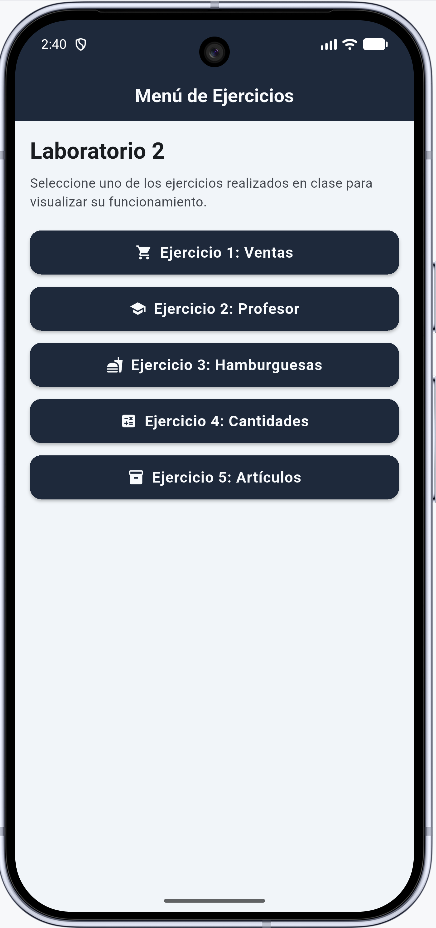
\includegraphics[width=0.4\textwidth]{main.png}
    \vspace{0.5cm} \\
    \textit{Ejecución de la Pantalla Principal}
\end{center}

\newpage
\subsection{Problema 1: Cálculo de IVA y Descuento}
\textbf{Descripción:}\\
Indicaciones al ejercicio en clase: calcular el iva de 15\%, si las compras superan 2000\$ al cliente se agrega un descuento del 20\%, mostrar tanto el sueldo a ganar del vendedor y la factura de la venta de productos.

\subsubsection{Pseudocódigo}
\begin{verbatim}
Inicio
  Leer subtotalCompra
  Leer sueldoBaseVendedor
  Leer porcentajeComisionVenta
  
  iva = subtotalCompra * 0.15
  totalConIva = subtotalCompra + iva
  
  descuento = 0
  Si subtotalCompra > 2000 Entonces
    descuento = totalConIva * 0.20
  FinSi
  
  totalFactura = totalConIva - descuento
  
  comision = subtotalCompra * (porcentajeComisionVenta / 100)
  sueldoVendedor = sueldoBaseVendedor + comision
  
  Imprimir "--- Factura del Cliente ---"
  Imprimir "Subtotal: $", subtotalCompra
  Imprimir "IVA (15%): $", iva
  Imprimir "Descuento: $", descuento
  Imprimir "Total a Pagar: $", totalFactura
  
  Imprimir "--- Sueldo Vendedor ---"
  Imprimir "Sueldo a ganar: $", sueldoVendedor
Fin
\end{verbatim}

\subsubsection{Diagrama Nassi-Shneiderman}
\vspace{0.5cm}
\begin{center}
\begin{struktogramm}(150, 100)
  \assign{Leer \texttt{subtotalCompra}, \texttt{sueldoBaseVendedor}, \texttt{porcentajeComisionVenta}}
  \assign{\texttt{iva} $\gets$ \texttt{subtotalCompra} * 0.15}
  \assign{\texttt{totalConIva} $\gets$ \texttt{subtotalCompra} + \texttt{iva}}
  \assign{\texttt{descuento} $\gets$ 0}
  \ifthenelse[15]{1}{1}{\texttt{subtotalCompra} $>$ 2000}{\textbf{Sí}}{\textbf{No}}
    \assign{\texttt{descuento} $\gets$ \texttt{totalConIva} * 0.20}
  \change
  \ifend
  \assign{\texttt{totalFactura} $\gets$ \texttt{totalConIva} - \texttt{descuento}}
  \assign{\texttt{comision} $\gets$ \texttt{subtotalCompra} * (\texttt{porcentajeComisionVenta} / 100)}
  \assign{\texttt{sueldoVendedor} $\gets$ \texttt{sueldoBaseVendedor} + \texttt{comision}}
  \assign{Imprimir \texttt{totalFactura}, \texttt{sueldoVendedor}}
\end{struktogramm}
\end{center}
\vspace{1.5cm}

\subsubsection{Código }
\begin{maccode}{lib/model/factura\_model.dart}
  void procesarFactura(double subtotal, double sueldoBase, double comisionPorcentaje) {
    double iva = subtotal * 0.15;
    double totalConIva = subtotal + iva;
    
    double descuento = 0.0;
    if (subtotal > 2000) {
      descuento = totalConIva * 0.20;
    }
    double totalFactura = totalConIva - descuento;
    
    double comision = subtotal * (comisionPorcentaje / 100);
    double sueldoVendedor = sueldoBase + comision;
    // Retornar o actualizar estado con los resultados
  }
\end{maccode}
\vspace{0.3cm}
\textbf{Descripción:} La función recibe el subtotal de la compra y los datos salariales del vendedor. Calcula el IVA, evalúa si aplica el descuento por compras mayores a 2000, y finalmente determina el salario del vendedor basándose en su sueldo base y comisión.

\subsubsection{Ejecución}
\begin{center}
    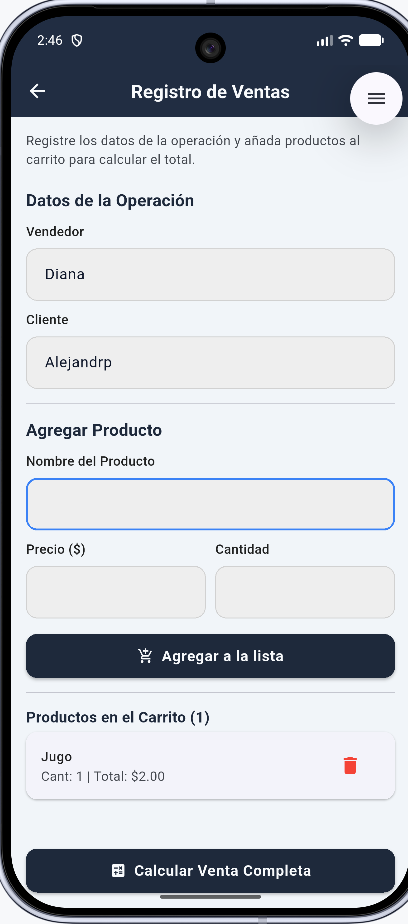
\includegraphics[width=0.4\textwidth]{img_prob1.png}
    \vspace{0.5cm} \\
    \textit{Ejecución del Problema 1}
\end{center}

\subsubsection{Salida Esperada}
\begin{center}
    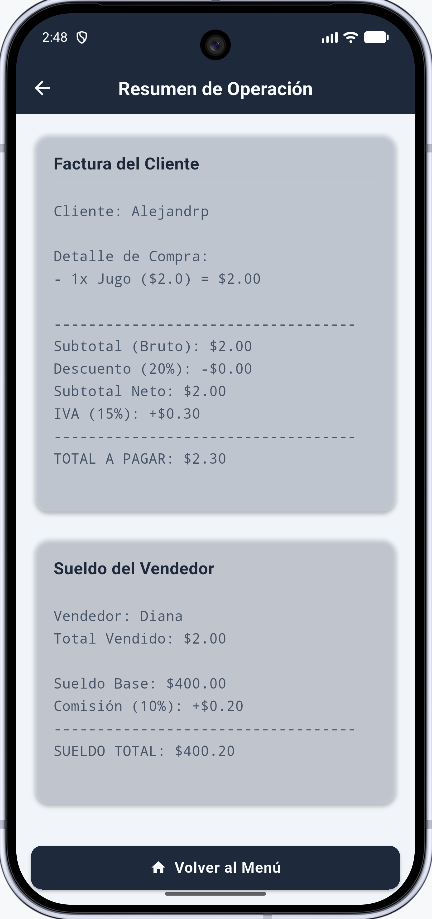
\includegraphics[width=0.4\textwidth]{img_prob1s.png}
    \vspace{0.5cm} \\
    \textit{Salida del Problema 1}
\end{center}

\newpage
\subsection{Problemas 2}

\subsubsection{Ejercicio 4.1: Incremento salarial}
\textbf{Descripción:}\\
Un profesor tiene un salario inicial de \$1500, y recibe un incremento de 10 \% anual durante 6 años. ¿Cuál es su salario al cabo de 6 años? ¿Qué salario ha recibido en cada uno de los 6 años? Realice el algoritmo utilizando el ciclo apropiado.

\textbf{Pseudocódigo:}
\begin{verbatim}
Inicio
  salario = 1500
  Para año = 1 Hasta 6 Hacer
    incremento = salario * 0.10
    salario = salario + incremento
    Imprimir "Salario recibido en el año ", año, ": $", salario
  FinPara
  Imprimir "El salario final al cabo de los 6 años es: $", salario
Fin
\end{verbatim}

\textbf{Diagrama Nassi-Shneiderman:}
\vspace{0.5cm}
\begin{center}
\begin{struktogramm}(140, 60)
  \assign{\texttt{salario} $\gets$ 1500}
  \while{Para \texttt{año} = 1 Hasta 6}
    \assign{\texttt{incremento} $\gets$ \texttt{salario} * 0.10}
    \assign{\texttt{salario} $\gets$ \texttt{salario} + \texttt{incremento}}
    \assign{Imprimir "Salario año ", \texttt{año}, ": \$", \texttt{salario}}
  \whileend
  \assign{Imprimir "Salario final: \$", \texttt{salario}}
\end{struktogramm}
\end{center}
\vspace{1.5cm}

\textbf{Código:}
\begin{maccode}{lib/model/profesor\_model.dart}
  void calcularIncrementos() {
    double salario = 1500.0;
    for (int i = 1; i <= 6; i++) {
      double incremento = salario * 0.10;
      salario += incremento;
      print("Salario año $i: $salario");
    }
    // El salario final al cabo de 6 años está en 'salario'
  }
\end{maccode}
\vspace{0.3cm}
\textbf{Descripción:} A través de un bucle \texttt{for} que itera 6 veces, el algoritmo toma el salario base y calcula de forma acumulativa el 10\% de incremento año tras año.

\subsubsection{Ejecución}
\begin{center}
    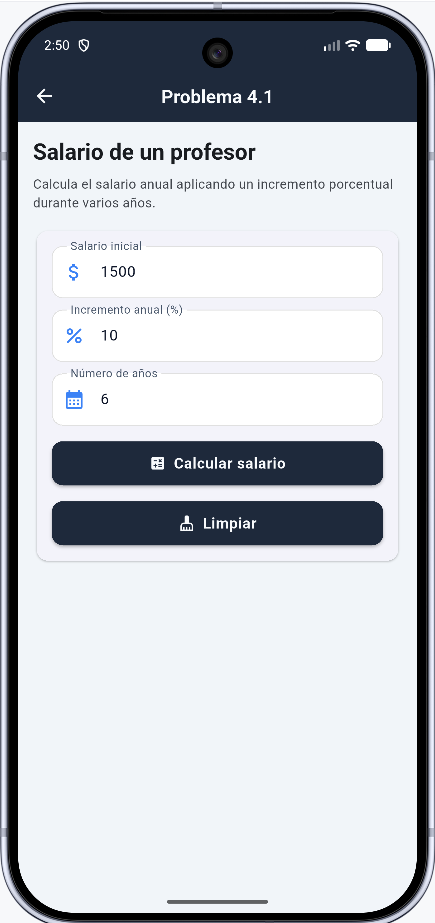
\includegraphics[width=0.4\textwidth]{img_prob2.png}
    \vspace{0.5cm} \\
    \textit{Ejecución del Problema 2}
\end{center}

\subsubsection{Salida Esperada}
\begin{center}
    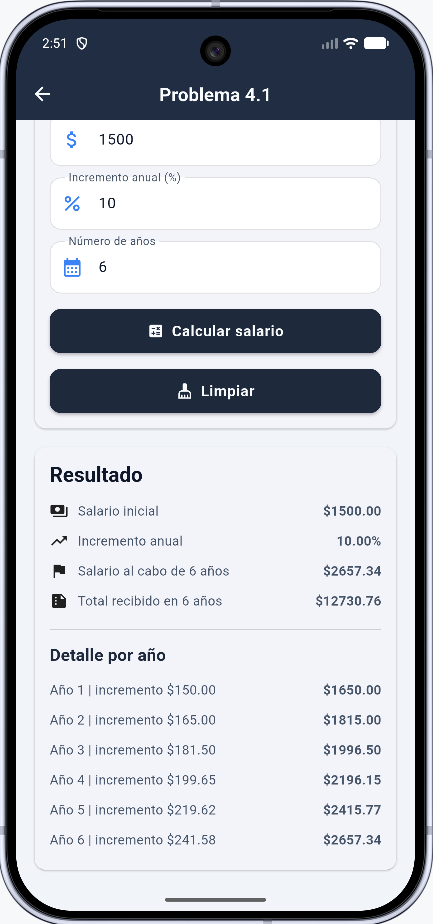
\includegraphics[width=0.4\textwidth]{img_prob2s.png}
    \vspace{0.5cm} \\
    \textit{Salida del Problema 2}
\end{center}


\newpage
\subsubsection{Ejercicio 4.2: El náufrago satisfecho}
\textbf{Descripción:}\\
“El náufrago satisfecho” ofrece hamburguesas sencillas (S) a \$20, dobles (D) a \$25 y triples (T) a \$28. La empresa acepta tarjetas de crédito con un cargo de 5 \% sobre la compra. Suponiendo que los clientes adquieren N hamburguesas, realice el algoritmo para determinar cuánto deben pagar.

\textbf{Pseudocódigo:}
\begin{verbatim}
Inicio
  Leer N // Cantidad de hamburguesas
  Leer usaTarjeta // Verdadero o Falso
  totalCosto = 0
  
  Para i = 1 Hasta N Hacer
    Leer tipoHamburguesa // Puede ser S, D, T
    Si tipoHamburguesa == "S" Entonces
      totalCosto = totalCosto + 20
    Sino Si tipoHamburguesa == "D" Entonces
      totalCosto = totalCosto + 25
    Sino Si tipoHamburguesa == "T" Entonces
      totalCosto = totalCosto + 28
    FinSi
  FinPara
  
  cargoTarjeta = 0
  Si usaTarjeta == Verdadero Entonces
    cargoTarjeta = totalCosto * 0.05
  FinSi
  
  totalAPagar = totalCosto + cargoTarjeta
  Imprimir "Subtotal hamburguesas: $", totalCosto
  Imprimir "Cargo por tarjeta: $", cargoTarjeta
  Imprimir "Total a Pagar: $", totalAPagar
Fin
\end{verbatim}

\textbf{Diagrama Nassi-Shneiderman:}
\vspace{0.5cm}
\begin{center}
\begin{struktogramm}(140, 110)
  \assign{Leer \texttt{N}, \texttt{usaTarjeta}}
  \assign{\texttt{totalCosto} $\gets$ 0}
  \while{Para \texttt{i} = 1 Hasta \texttt{N}}
    \assign{Leer \texttt{tipoHamburguesa}}
    \ifthenelse[15]{1}{1}{\texttt{tipoHamburguesa} == 'S'}{\textbf{Sí}}{\textbf{No}}
      \assign{\texttt{totalCosto} $\gets$ \texttt{totalCosto} + 20}
    \change
      \ifthenelse[15]{1}{1}{\texttt{tipoHamburguesa} == 'D'}{\textbf{Sí}}{\textbf{No}}
        \assign{\texttt{totalCosto} $\gets$ \texttt{totalCosto} + 25}
      \change
        \ifthenelse[15]{1}{1}{\texttt{tipoHamburguesa} == 'T'}{\textbf{Sí}}{\textbf{No}}
          \assign{\texttt{totalCosto} $\gets$ \texttt{totalCosto} + 28}
        \change
        \ifend
      \ifend
    \ifend
  \whileend
  \assign{\texttt{cargoTarjeta} $\gets$ 0}
  \ifthenelse[15]{1}{1}{\texttt{usaTarjeta} == Verdadero}{\textbf{Sí}}{\textbf{No}}
    \assign{\texttt{cargoTarjeta} $\gets$ \texttt{totalCosto} * 0.05}
  \change
  \ifend
  \assign{\texttt{totalAPagar} $\gets$ \texttt{totalCosto} + \texttt{cargoTarjeta}}
  \assign{Imprimir \texttt{totalAPagar}}
\end{struktogramm}
\end{center}
\vspace{2.5cm}

\textbf{Código:}
\begin{maccode}{lib/model/hamburguesas\_model.dart}
  void calcularPago(List<String> hamburguesasCompradas, bool usaTarjeta) {
    double totalCosto = 0.0;
    for (String tipo in hamburguesasCompradas) {
      if (tipo == 'S') totalCosto += 20;
      else if (tipo == 'D') totalCosto += 25;
      else if (tipo == 'T') totalCosto += 28;
    }
    
    double cargoTarjeta = usaTarjeta ? (totalCosto * 0.05) : 0.0;
    double totalAPagar = totalCosto + cargoTarjeta;
  }
\end{maccode}
\vspace{0.3cm}
\textbf{Descripción:} La función recibe una lista con los tipos de hamburguesas y un valor booleano para la tarjeta. Itera la lista sumando los costos según el tipo, y al final aplica un recargo del 5\% sobre el acumulado si es un pago con tarjeta.

\subsubsection{Ejecución}
\begin{center}
    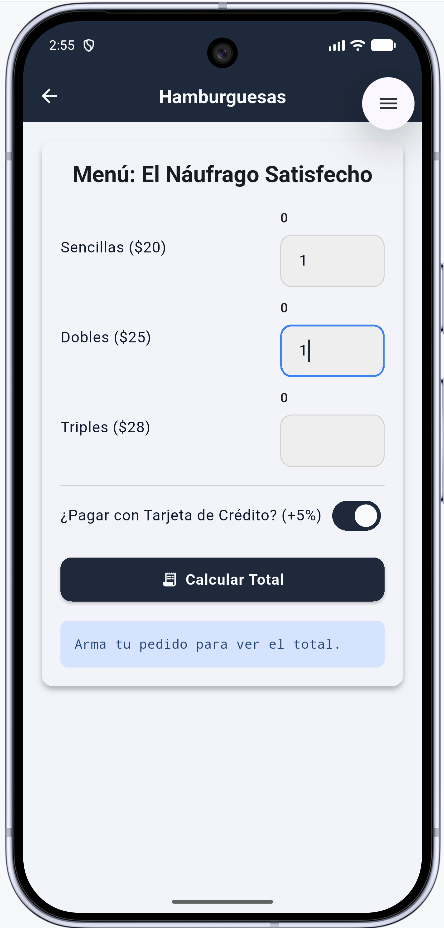
\includegraphics[width=0.4\textwidth]{img_prob4_2.png}
    \vspace{0.5cm} \\
    \textit{Ejecución y salida del Problema 3}
\end{center}

\subsubsection{Salida Esperada}
\begin{center}
    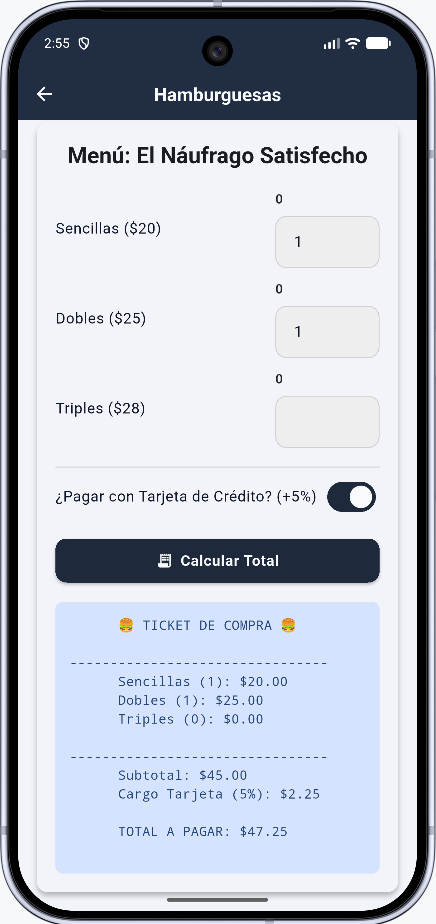
\includegraphics[width=0.4\textwidth]{img_prob4_2s.png}
    \vspace{0.5cm} \\
    \textit{Salida del Problema 3}
\end{center}



\newpage
\subsubsection{Ejercicio 4.3: Contar cantidades}
\textbf{Descripción:}\\
Se requiere un algoritmo para determinar, de N cantidades, cuántas son cero, cuántas son menores a cero, y cuántas son mayores a cero. Realice el algoritmo utilizando el ciclo apropiado.

\textbf{Pseudocódigo:}
\begin{verbatim}
Inicio
  Leer N // Número total de cantidades
  contadorCeros = 0
  contadorMenoresCero = 0
  contadorMayoresCero = 0
  
  Para i = 1 Hasta N Hacer
    Leer cantidad
    Si cantidad == 0 Entonces
      contadorCeros = contadorCeros + 1
    Sino Si cantidad < 0 Entonces
      contadorMenoresCero = contadorMenoresCero + 1
    Sino
      contadorMayoresCero = contadorMayoresCero + 1
    FinSi
  FinPara
  
  Imprimir "Cantidades iguales a cero: ", contadorCeros
  Imprimir "Cantidades menores a cero: ", contadorMenoresCero
  Imprimir "Cantidades mayores a cero: ", contadorMayoresCero
Fin
\end{verbatim}

\textbf{Diagrama Nassi-Shneiderman:}
\vspace{0.5cm}
\begin{center}
\begin{struktogramm}(140, 90)
  \assign{Leer \texttt{N}}
  \assign{\texttt{ceros} $\gets$ 0, \texttt{menores} $\gets$ 0, \texttt{mayores} $\gets$ 0}
  \while{Para \texttt{i} = 1 Hasta \texttt{N}}
    \assign{Leer \texttt{cantidad}}
    \ifthenelse[15]{1}{1}{\texttt{cantidad} == 0}{\textbf{Sí}}{\textbf{No}}
      \assign{\texttt{ceros} $\gets$ \texttt{ceros} + 1}
    \change
      \ifthenelse[15]{1}{1}{\texttt{cantidad} $<$ 0}{\textbf{Sí}}{\textbf{No}}
        \assign{\texttt{menores} $\gets$ \texttt{menores} + 1}
      \change
        \assign{\texttt{mayores} $\gets$ \texttt{mayores} + 1}
      \ifend
    \ifend
  \whileend
  \assign{Imprimir \texttt{ceros}, \texttt{menores}, \texttt{mayores}}
\end{struktogramm}
\end{center}
\vspace{1.5cm}

\textbf{Código:}
\begin{maccode}{lib/model/cantidades\_model.dart}
  void analizarCantidades(List<int> cantidades) {
    int ceros = 0, menores = 0, mayores = 0;
    
    for (int cantidad in cantidades) {
      if (cantidad == 0) ceros++;
      else if (cantidad < 0) menores++;
      else mayores++;
    }
    // Retorna o almacena los contadores
  }
\end{maccode}
\vspace{0.3cm}
\textbf{Descripción:} Se recorre una lista de números evaluando cada elemento mediante condicionales \texttt{if-else} para determinar si es neutro (cero), negativo o positivo, incrementando el contador correspondiente en cada caso.

\subsubsection{Ejecución}
\begin{center}
    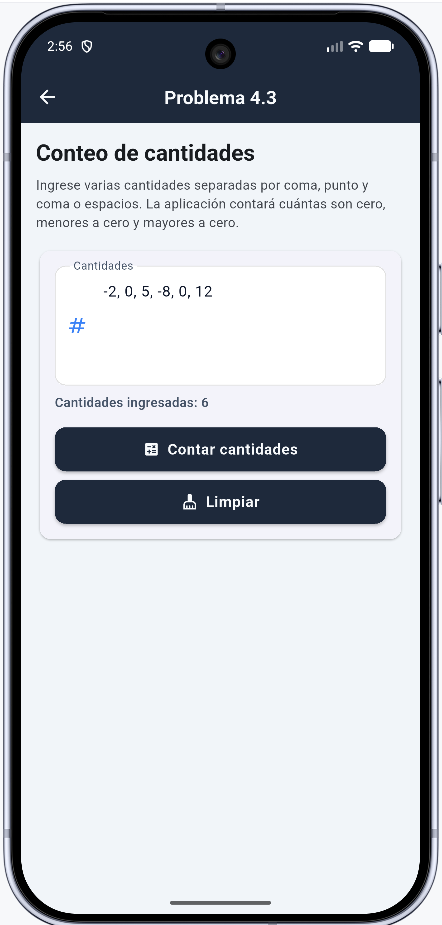
\includegraphics[width=0.4\textwidth]{img_prob4.png}
    \vspace{0.5cm} \\
    \textit{Ejecución y salida del Problema 4}
\end{center}

\subsubsection{Salida Esperada}
\begin{center}
    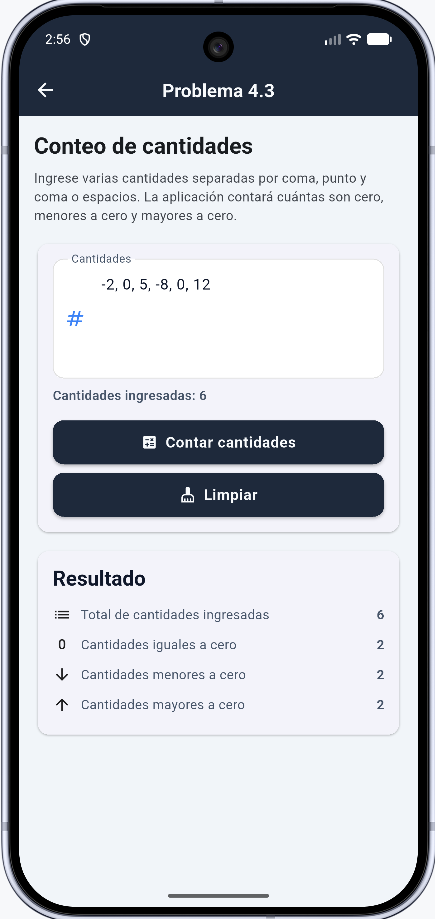
\includegraphics[width=0.4\textwidth]{img_prob4s.png}
    \vspace{0.5cm} \\
    \textit{Salida del Problema 4}
\end{center}


\newpage
\subsubsection{Ejercicio 4.8: Promoción de artículos}
\textbf{Descripción:}\\
Realice el algoritmo para determinar cuánto pagará una persona que adquiere N artículos, los cuales están de promoción:
- Precio >= \$200: descuento de 15\%
- \$100 < precio < \$200: descuento de 12\%
- Precio <= \$100: descuento de 10\%
Muestre el costo y descuento de cada artículo, y cuánto pagará por el total.

\textbf{Pseudocódigo:}
\begin{verbatim}
Inicio
  Leer N // Cantidad de artículos
  totalPagoGlobal = 0
  
  Para i = 1 Hasta N Hacer
    Leer precioArticulo
    descuentoArticulo = 0
    
    Si precioArticulo >= 200 Entonces
      descuentoArticulo = precioArticulo * 0.15
    Sino Si precioArticulo > 100 Entonces
      descuentoArticulo = precioArticulo * 0.12
    Sino
      descuentoArticulo = precioArticulo * 0.10
    FinSi
    
    precioFinalArticulo = precioArticulo - descuentoArticulo
    totalPagoGlobal = totalPagoGlobal + precioFinalArticulo
    
    Imprimir "Artículo ", i
    Imprimir "  Precio original: $", precioArticulo
    Imprimir "  Descuento: $", descuentoArticulo
    Imprimir "  Precio final: $", precioFinalArticulo
  FinPara
  
  Imprimir "Total a pagar por todos los artículos: $", totalPagoGlobal
Fin
\end{verbatim}

\textbf{Diagrama Nassi-Shneiderman:}
\vspace{0.5cm}
\begin{center}
\begin{struktogramm}(150, 100)
  \assign{Leer \texttt{N}}
  \assign{\texttt{totalPagoGlobal} $\gets$ 0}
  \while{Para \texttt{i} = 1 Hasta \texttt{N}}
    \assign{Leer \texttt{precioArticulo}}
    \assign{\texttt{descuentoArticulo} $\gets$ 0}
    \ifthenelse[15]{1}{1}{\texttt{precioArticulo} $\ge$ 200}{\textbf{Sí}}{\textbf{No}}
      \assign{\texttt{descuentoArticulo} $\gets$ \texttt{precioArticulo} * 0.15}
    \change
      \ifthenelse[15]{1}{1}{\texttt{precioArticulo} $>$ 100}{\textbf{Sí}}{\textbf{No}}
        \assign{\texttt{descuentoArticulo} $\gets$ \texttt{precioArticulo} * 0.12}
      \change
        \assign{\texttt{descuentoArticulo} $\gets$ \texttt{precioArticulo} * 0.10}
      \ifend
    \ifend
    \assign{\texttt{precioFinalArticulo} $\gets$ \texttt{precioArticulo} - \texttt{descuentoArticulo}}
    \assign{\texttt{totalPagoGlobal} $\gets$ \texttt{totalPagoGlobal} + \texttt{precioFinalArticulo}}
  \whileend
  \assign{Imprimir \texttt{totalPagoGlobal}}
\end{struktogramm}
\end{center}
\vspace{1.5cm}

\textbf{Código:}
\begin{maccode}{lib/model/promocion\_model.dart}
  void procesarArticulos(List<double> precios) {
    double totalGlobal = 0.0;
    
    for (double precio in precios) {
      double descuento = 0.0;
      if (precio >= 200) descuento = precio * 0.15;
      else if (precio > 100) descuento = precio * 0.12;
      else descuento = precio * 0.10;
      
      double precioFinal = precio - descuento;
      totalGlobal += precioFinal;
    }
    // 'totalGlobal' contiene lo que se pagará en total
  }
\end{maccode}
\vspace{0.3cm}
\textbf{Descripción:} La lógica analiza el precio individual de cada artículo iterado para aplicarle su descuento respectivo. Resta el descuento al costo base y va acumulando los precios resultantes en una variable global que dictará el total a pagar.

\subsubsection{Ejecución}
\begin{center}
    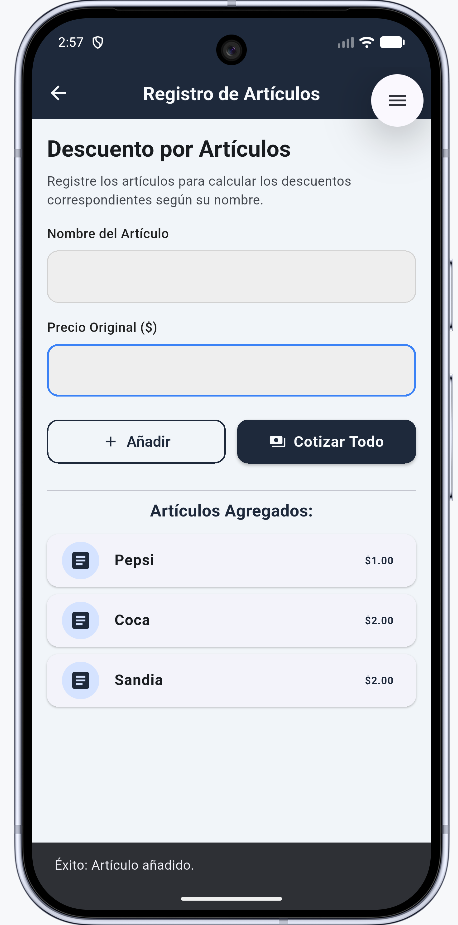
\includegraphics[width=0.4\textwidth]{img_prob5.png}
    \vspace{0.5cm} \\
    \textit{Ejecución y salida del Problema 5}
\end{center}

\subsubsection{Salida Esperada}
\begin{center}
    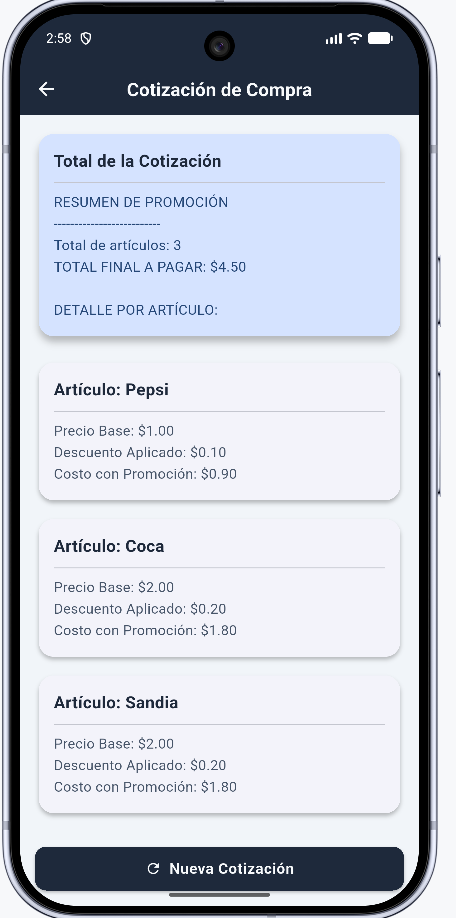
\includegraphics[width=0.4\textwidth]{img_prob5s.png}
    \vspace{0.5cm} \\
    \textit{Salida del Problema 5}
\end{center}

\newpage
\section{Conclusiones}
\begin{itemize}
    \item La implementación de un \textit{Splash screen} mejora significativamente la experiencia del usuario, ocultando tiempos de carga iniciales bajo una estética de marca que aplica un componente UI fundamental en el desarrollo móvil.
    \item Las instrucciones de navegación de Flutter, como \texttt{push}, \texttt{pop} y \texttt{pushNamed}, proveen un control exhaustivo sobre la pila de interfaces, logrando transiciones asíncronas fiables entre los ejercicios propuestos.
    \item Se completó con éxito el análisis secuencial y lógico de todos los problemas matemáticos y financieros a través del diseño de pseudocódigos altamente estructurados, validando su comportamiento antes de escribir instrucciones propias de un marco de trabajo.
\end{itemize}

\section{Referencias}
\begin{itemize}
  \item Google (2024). \textit{Flutter Documentation}. Recuperado de \url{https://docs.flutter.dev/}
  \item Google (2024). \textit{Dart Language Overview}. Recuperado de \url{https://dart.dev/overview}
  \item Google (2024). \textit{Android Studio User Guide}. Recuperado de \url{https://developer.android.com/studio/intro}
\end{itemize}

\section{Anexos}
\subsection{Repositorio de código fuente}

\subsubsection{Enlace principal}
\begin{itemize}
  \item \url{https://github.com/LeonelTQL/moviles/tree/main/pry_lab2}
\end{itemize}

\end{document}
